\chapter{实验评估}

本章将详细阐述为评估\tool 所进行的实验验证,并讨论分析实验的结果。本章将首先介绍所设计的五个实验问题,包括准确性、削弱性、敏感度、通用性及实用性的验证;再逐一展示五个问题的实验结果,并讨论分析其原因及意义;最后,基于实验验证的结果,讨论\tool 的局限性以及实际价值。

\section{实验问题设计}
本文从准确性、削弱性、敏感度、通用性及实用性五个方面设计了以下五个研究问题,以尽可能全面地验证并评估\tool 。

\begin{itemize}[leftmargin=*]
\item \textbf{RQ6 准确性评估:}与已有的基于启发式的方法相比,\tool 查找漏洞补丁的准确性如何?与两个商业漏洞数据库相比,\tool 提供的漏洞补丁的准确性又如何呢?这个问题旨在探究\tool 的准确性。(见章节\ref{sec:accuracy-evaluation})
\item \textbf{RQ7 削弱性分析:}\tool 中各个步骤及设计有着怎么样的效果或必要性?如果去除或削弱\tool 中的某些环节,对于\tool 的结果会有怎么样的影响?这个问题旨在评估\tool 中各个步骤及设计的实际效果及必要性。(Sec.\ref{sec:ablation})
\item \textbf{RQ8 敏感度分析:}\tool 的准确性对\tool 中参数的敏感性如何?这个问题旨在评估\tool 的健壮性及鲁棒性,探究tool 中的参数是否对\tool 的准确性有过大影响。 (见章节\ref{sec:sensitivity})
\item \textbf{RQ9 通用性分析:}\tool 在更大范围的开源软件漏洞上表现如何? 这个问题旨在评估\tool 的通用性。(见章节\ref{sec:sensitivity})
\item \textbf{RQ10 实用性分析:}\tool 在实际使用中表现如何?这个问题旨在评估\tool 在实际使用中实用性。(见章节\ref{sec:generality})
\end{itemize}

为解答以上实验问题,本章的实验验证将继续采用经验研究(见章节\ref{sec:accuracy})中使用的评估指标,即Not Found、Precision(精确率)、Recall(召回率)和 F1-Score(F1值)。本章的实验验证还将继续使用在经验研究(见章节\ref{sec:study})中构建了深度数据集,以探究\textbf{RQ6 准确性验证}、\textbf{RQ7 削弱性分析}和\textbf{RQ8 敏感度分析}。

对于\textbf{RQ9 通用性分析},本章将另外构造两个范围更大的数据集来进行验证。此外,本章还进行了用户研究,通过评估用户分别在有和没有\tool 辅助下查找补丁的用时和准确性,并收集用户反馈以探究\textbf{RQ10 实用性分析}。


\section{RQ6:准确性验证}\label{sec:accuracy-evaluation}

为了评估\tool 的准确性,本节将\tool 分别与三种基于启发式的方法和两个商业漏洞数据库($DB_A$和$DB_B$)进行比较,并通过人工进一步分析了\tool 中误报和漏报的原因。

\subsection{与基于启发式规则的方法对比}
本节首先选择了两种被广泛使用的启发式方法(\textbf{检索NVD References}和\textbf{检索GitHub Commits}),此外,还将这前种启发式方法结合为第三种启发式方法(\textbf{检索NVD以及GitHub})。

\textbf{检索NVD References:}检索NVD平台上该漏洞“Reference”字段中的引用信息以获取补丁提交\cite{duan2019automating,li2016vulpecker,li2018vuldeepecker}。如图\ref{fig:CVE-2019-18841}所示为NVD平台上CVE-2019-18841的引用信息\footnote{https://nvd.nist.gov/vuln/detail/CVE-2019-18841},可以从中提取出补丁提交“\url{https://github.com/ankane/chartkick/commit/b810936bbf687bc74c5b6dba72d2397a399885fa}”。
\begin{figure*}[h]
    \centering
    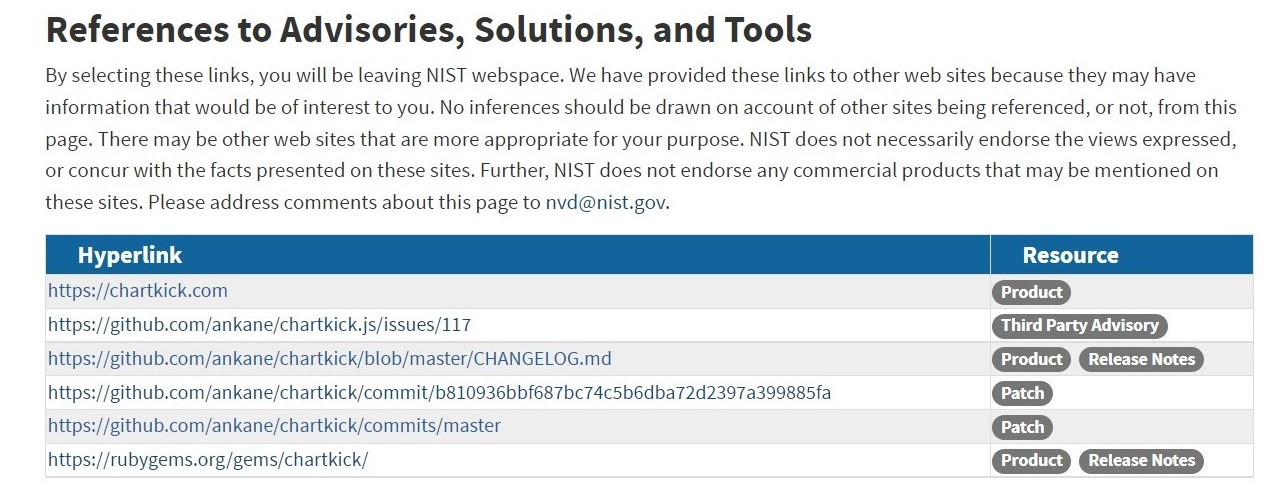
\includegraphics[scale=0.44]{fig/NVD-2019-18841}
    %\vspace{-10pt}
    \caption{NVD平台CVE-2019-18841的引用信息}\label{fig:CVE-2019-18841}
\end{figure*}

\textbf{检索GitHub Commits:}检索GitHub中,检索带有CVE标识符的代码提交\cite{you2017semfuzz,Wang2020empirical}。如图\ref{fig:commitmessage}所示,提交信息(Commit Message)\footnote{https://github.com/apache/tomcat80/commit/2c9d8433bd3247a2856d4b255}为“Fix \url{https://bz.apache.org/bugzilla/show_bug.cgi?id=62343} Make CORS filter defaults more secure. This is the fix for CVE-2018-8014.”,漏洞标识符“CVE-2018-8014”出现在该提交中。以“CVE-2018-8014”为输入,通过检索Github获取该提交,作为漏洞CVE-2018-8014的补丁。
\begin{figure*}[h]
    \centering
    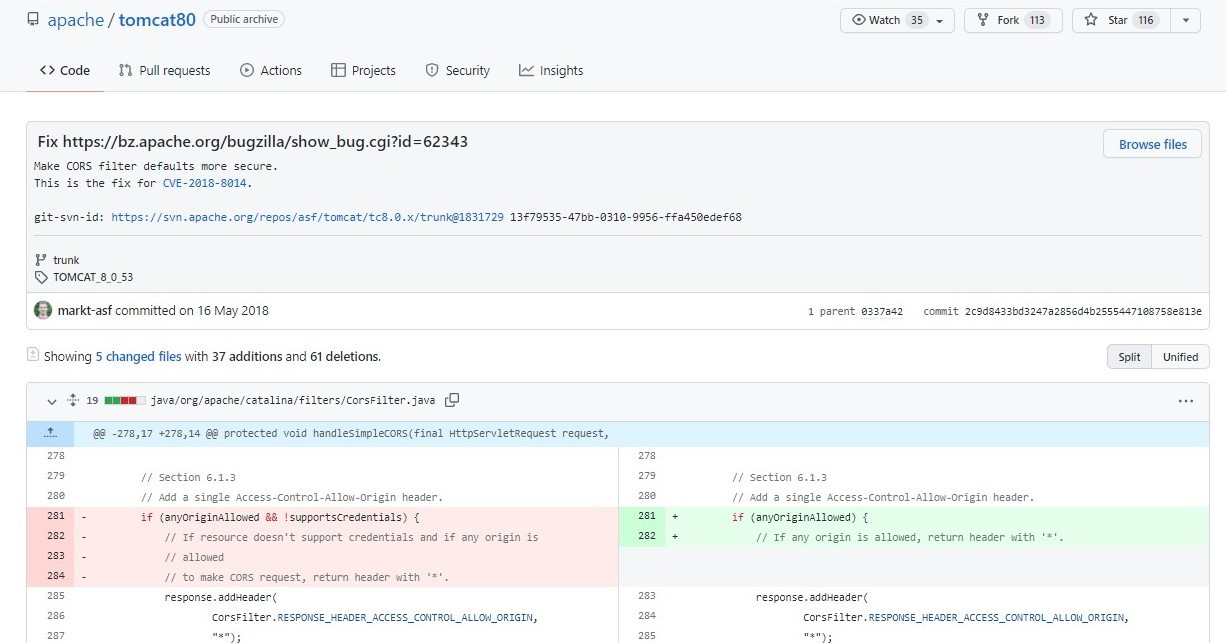
\includegraphics[scale=0.45]{fig/CVE in commit message.jpg}
    %\vspace{-10pt}
    \caption{CVE-2018-8014标识符出现在提交中}\label{fig:commitmessage}
\end{figure*}

\textbf{检索NVD 以及GitHub:}将前两种启发式方法结合为第三种启发式方法,即检索NVD References以及GitHub Commits。

\begin{table*}[h]
    \centering
    % \footnotesize
    \small
    \caption{\tool VS. 已有的基于启发式的方法}\label{table:heuristic}
    %\vspace{-10pt}
    \begin{tabular}{|*{1}{C{4.2em}}|*{1}{C{2.0em}}|*{1}{C{4.9em}}*{3}{C{2.0em}}|*{1}{C{4.9em}}*{3}{C{2.0em}}|}
    % \begin{tabular}{|c|c|cccc|cccc|}
    \noalign{\hrule height 1pt}
    \multirow{2}{*}{映射类型} & \multirow{2}{*}{数量} &  \multicolumn{4}{c|}{检索NVD References} & \multicolumn{4}{c|}{检索GitHub Commits}\\\cline{3-10}
    & & Not Found & Pre. & Rec. & F1 & Not Found & Pre. & Rec. & F1 \\
    \noalign{\hrule height 1pt}
    1:1 (SP) & 567 &	285 (50.3\%) & 0.973 & 0.986 & 0.977 &	472 (83.2\%) & 0.416 & 0.642 & 0.471 	 \\
    1:$i$ (MEP) &195 &	125 (64.1\%) & 0.932 & 0.925 & 0.921 &	162 (83.1\%) & 0.472 & 0.490 & 0.452 	 \\
    1:$n$ (MP) & 101 &	68 (67.3\%) & 0.980 & 0.552 & 0.683 &	73 (72.3\%) & 0.536 & 0.445 & 0.461 	 \\
    1:$n$ (MB) & 372 &	244 (65.6\%) & 0.979 & 0.416 & 0.546 &	246 (66.1\%) & 0.445 & 0.236 & 0.284 	 \\
    1:$n$ (MR) & 60 &	46 (76.7\%) & 1.000 & 0.708 & 0.794 &	37 (61.7\%) & 0.627 & 0.345 & 0.413 	 \\\hline
    Total & 1,295 &	    768 (59.3\%) & 0.970 & 0.805 & 0.842 &	990 (76.4\%) & 0.461 & 0.417 & 0.386 	 \\
    \noalign{\hrule height 1pt}
    \multirow{2}{*}{映射类型} & \multirow{2}{*}{数量} &  \multicolumn{4}{c|}{检索NVD以及GitHub} & \multicolumn{4}{c|}{\tool}\\\cline{3-10}
    & & Not Found & Pre. & Rec. & F1 & Not Found & Pre. & Rec. & F1 \\
    \noalign{\hrule height 1pt}
    1:1 (SP) & 567 &	222 (39.2\%) & 0.839 & 0.930 & 0.864 & 102 (18.0\%) & 0.860 & 0.951 & 0.881 \\
    1:$i$ (MEP) &195 &	104 (53.3\%) & 0.821 & 0.867 & 0.820 & 6 (3.1\%) & 0.886 & 0.918 & 0.888 \\
    1:$n$ (MP) & 101 &	52 (51.5\%) & 0.779 & 0.605 & 0.647  & 20 (19.8\%) & 0.872 & 0.741 & 0.761\\
    1:$n$ (MB) & 372 &	171 (46.0\%) & 0.704 & 0.393 & 0.465 & 23 (6.2\%) & 0.861 & 0.788 & 0.795\\
    1:$n$ (MR) & 60 &	27 (45.0\%) & 0.801 & 0.539 & 0.604  & 4 (6.7\%) & 0.831 & 0.620 & 0.659 \\\hline
    Total & 1,295 &	    576 (44.5\%) & 0.793 & 0.732 & 0.720 & 155 (12.0\%) & 0.864 & 0.864 & 0.837\\
    \noalign{\hrule height 1pt}
    \end{tabular}
\end{table*}

表\ref{table:heuristic}显示了三种启发式方法与\tool 的准确率对比结果。可以发现,对于很大一部分漏洞,三种启发式方法都无法找到其补丁。深度数据集的1295个漏洞中,基于检索NVD References的启发式方法,\tocheck{768(59.3\%)}的漏洞无法找到补丁;基于检索GitHub Commits的启发式方法,\tocheck{990(76.4\%)}的漏洞无法找到补丁;基于检索NVD以及GitHub的启发式方法,\tocheck{576(44.5\%)}的漏洞无法找到补丁;然而,仅\tocheck{155(12.0\%)}漏洞的补丁无法被\tool 找到。

由于NVD References中引用信息都经过人工核对,References中引用信息的置信度比较高,所以基于检索NVD References的启发式方法具有较高的精确率(\tocheck{0.970})。但对于一对多映射关系的CVE,基于检索NVD References的启发式方法召回率就比较低,分别为\tocheck{0.552、0.416和0.708}。这也反映出NVD平台漏洞补丁的不完整情况。基于检索GitHub Commits的启发式方法具有较低的精确率和召回率,分别为\tocheck{0.461}和\tocheck{0.417},而基于检索NVD以及GitHub的启发式方法中和了前两种方法的精确率和召回率分别为\tocheck{0.793}和\tocheck{0.732}。

与基于检索NVD References的启发式方法对比,\tool 的精确率更低,但拥有更高的召回率和相似的F1值;尤其是对于\textit{MP}和\textit{MB}类型的CVE,\tool 的召回率也明显更高。考虑到\tool 找到补丁的漏洞数比第一种启发式方法多出\tocheck{116.3\%},\tool 中轻微的准确率降低是可以接受的。

与基于检索GitHub Commits的启发式方法和基于检索NVD以及GitHub的启发式方法对比,\tool 在精确率、召回率和F1值上全面胜出。\tool 的F1值分别高出了\tocheck{116.8\%}和\tocheck{16.3\%}。

\begin{tcolorbox}[size=title,opacityfill=0.15]
Highlight:与现有的基于启发式的方法相比,\tool 将能找到补丁的漏洞数提高\tocheck{58.6\%}到\tocheck{273.8\%},同时,将F1值提高\tocheck{116.8\%}。
\end{tcolorbox}


\subsection{与商业漏洞数据库对比}
% 考虑到漏洞数据库$DB_A$和$DB_B$并非由工具自动化构建,构建的过程涉及了大量人工工作,并不可知且无法量化,无法进行公平的比较。
% 本节与商业漏洞数据库$DB_A$和$DB_B$进行比较的并非为了证明\tool 或是$DB_A$和$DB_B$的优劣,因为

考虑到漏洞数据库$DB_A$和$DB_B$并非由工具自动化构建,构建的过程涉及了大量人工工作,因此,漏洞数据库$DB_A$和$DB_B$中漏洞信息具有较高的质量。本节将\tool 与数据库$DB_A$和$DB_B$进行对比,可以评估\tool 所达到的准确性水平。如果\tool 可以帮助改进或补充现有的商业漏洞数据库,也能体现\tool 的实用价值。

从表\ref{table:accuracy}和\ref{table:heuristic}可以看出,\tool 能找到补丁的漏洞数比$DB_A$和$DB_B$少了\tocheck{12.0\%},且精确率也分别低了\tocheck{6.4\%}和\tocheck{5.8\%}。这是因为漏洞数据库$DB_A$和$DB_B$构建过程中涉及了安全专家的人工工作,许多补丁由人工收集得来,难以被自动化工具找到。此外,收集的补丁还会经过安全专家验证,因此$DB_A$和$DB_B$也比自动化工具更高的准确率。

此外,\tool 的精确率、召回率和F1值分别为:0.864、0.864和0.837,$DB_A$ 的精确率、召回率和F1值分别为:0.923、0.748和0.793,$DB_B$ 的精确率、召回率和F1值分别为:0.917、0.730和0.771。可以发现\tool 的召回率比$DB_A$和$DB_B$高\tocheck{15.5\%和18.4\%},尤其是对于一对多映射的CVE,\tool 具有更高的召回率;\tool 的F1值也比$DB_A$和$DB_B$高\tocheck{5.5\%和8.6\%}。

这些结果表明,与漏洞数据库$DB_A$和$DB_B$相比,\tool 以较低的精确率和较少未找到补丁的漏洞为代价,拥有更为显着的召回率。这也说明,\tool 可用于补充现有漏洞数据库缺失的漏洞补丁数据。

\begin{tcolorbox}[size=title,opacityfill=0.15]
Highlight:\tool 具有比$DB_A$和$DB_B$高\tocheck{15.5\%和18.4\%}的召回率,以及高\tocheck{5.5\%到8.6\%}的F1值,但同时\tool 牺牲了\tocheck{6.4\%}的精确率和\tocheck{12.0\%}CVE的补丁。
\end{tcolorbox}

\subsection{漏报和误报分析}\label{sec:fpfn}

基于前两小节的实验结果,本小节旨在分析造成\tool 漏报和误报的原因,即\tool 未找到补丁或返回的补丁不正确的情形。

\textbf{漏报分析:} 漏报是指\tool 未能找到补丁或找全补丁,体现在召回率(Recall)小于1,以及Not Found不为0。通过人工分析\tool 未能找到补丁或找全补丁的CVE数据,本小节共总结出\tool 漏报的五个主要原因:
\begin{enumerate}
    \item [(1)] 对于一些年代久远的CVE,NVD、Debian和Red Hat中包含的引用信息比较少,有的引用信息甚至是失效的。这种情况下,\tool 无法构建完整的参考网络。例如,\tool 未能找到补丁的漏洞CVE-2011-1950,该漏洞在NVD\footnote{https://nvd.nist.gov/vuln/detail/CVE-2011-1950}中标记为“补丁(Patch)”和“供应商咨询(Vendor Advisory)”的关键参考链接已经失效,而这个链接中很有可能含有补丁。
    \item [(2)] NVD、Debian和Red Hat平台缺失关键参考链接(例如,问题链接(Issue URL)),\tool 便难以选出正确的补丁。例如,\tool 未能找到补丁的漏洞CVE-2018-14642,其问题报告\footnote{https://issues.redhat.com/browse/UNDERTOW-1430}不包含在任何一个知识源中,人工分析发现,基于此问题报告可以找到该漏洞的补丁\footnote{https://github.com/undertow-io/undertow/commit/c46b7b49c5a561731c84a76ee52244369af1af8a}。
    \item [(3)] 补丁的提交信息不包含CVE标识符,但与CVE描述具有语义相似性,自动化工具难以识别,但可通过人工识别。因此,\tool 的\tocheck{知识源扩增}步骤也未能找到这类型的补丁。例如,漏洞CVE-2019-10077\footnote{https://nvd.nist.gov/vuln/detail/CVE-2019-10077},代码提交\footnote{https://github.com/apache/jspwiki/commit/87c89f0405d6b31fc165358ce5d5bc4536e32a8a}为该漏洞的补丁,但提交信息中未提及CVE标识符,\tool 也未能找到该补丁。
    \item [(4)] GitHub平台用于检索代码提交的REST API仅返回1,000个结果,这会使\tool 在\tocheck{知识源扩增}步骤种错失一些补丁提交。
    \item [(5)] \tool 的补丁精选步骤中,只选择了一个具有最高连通度的补丁节点,其他已包含在参考链接网络中的正确补丁会被遗漏掉,这也造成了漏报。
\end{enumerate}


\textbf{误报分析:}漏报是指\tool 返回的结果非该漏洞的补丁,体现在精确率(Precision)小于1。通过人工分析\tool 返回错误补丁的CVE数据,本小节共总结出\tool 误报的两个主要原因:

\begin{enumerate}
    \item [(1)] 在讨论和解决漏洞时,相关人员也会引用引入漏洞的代码提交。由于\tool 缺乏对参考链接的上下文语义理解,\tool 错误地将其识别为补丁提交。例如,漏洞CVE-2020-5249,引入漏洞的代码提交\footnote{https://github.com/ethereum/go-ethereum/commit/fb9f7261ec51e38eedb454594fc19f00de1a6834}和修复漏洞的代码提交\footnote{https://github.com/ethereum/go-ethereum/commit/83e2761c3a13524bd5d6597ac08994488cf872ef}在同一问题报告(Issue Report)的评论中被引用。
    \item [(2)] 被引用的页面上列出了多对CVE及其问题和补丁。由于\tool 缺乏语义理解,其他CVE的补丁也可能会被\tool 错误地识别。例如,漏洞CVE-2018-15750,其补丁维护在发行说明(Release Note)\footnote{https://docs.saltstack.com/en/latest/topics/releases/2018.3.3.html}中,CVE-2018-15751的发行说明均被NVD、Debian和Red Hat引用。
\end{enumerate}  

\begin{tcolorbox}[size=title,opacityfill=0.15]
Highlight:通过人工分析共总结出\tool 漏报的五个主要原因和误报的两个主要原因,针对这些情形,可进一步提高\tool 的准确性。
\end{tcolorbox}

\section{RQ7:削弱性分析}\label{sec:ablation}

\begin{table*}[h]
    \centering
    \small
    \caption{\tool 削弱性分析结果(1)}\label{table:contribution}
    %\vspace{-10pt}
    \begin{tabular}{|*{1}{C{4.2em}}|*{1}{C{2.0em}}|*{1}{C{4.9em}}*{3}{C{2.0em}}|*{1}{C{4.9em}}*{3}{C{2.0em}}|}
    % \begin{tabular}{|c|c|cccc|cccc|}
    \noalign{\hrule height 1pt}
    \multirow{2}{*}{映射类型} & \multirow{2}{*}{数量} &  \multicolumn{4}{c|}{ \tool } & \multicolumn{4}{c|}{$v_1^1$: \tool w/o NVD} \\\cline{3-10}
    & & Not Found & Pre. & Rec. & F1 & Not Found & Pre. & Rec. & F1  \\
    \noalign{\hrule height 1pt}
    1:1 (SP) & 567 &	102 (18.0\%) & 0.860 & 0.951 & 0.881 &	286 (50.4\%) & 0.820 & 0.936 & 0.846  \\
    1:$i$ (MEP) &195 &	6 (3.1\%) & 0.886 & 0.918 & 0.888 &	    79 (40.5\%) & 0.882 & 0.935 & 0.886 	 \\
    1:$n$ (MP) & 101 &	20 (19.8\%) & 0.872 & 0.741 & 0.761 &	41 (40.6\%) & 0.881 & 0.728 & 0.766 	 \\
    1:$n$ (MB) & 372 &	23 (6.2\%) & 0.861 & 0.788 & 0.795 &	84 (22.6\%) & 0.876 & 0.780 & 0.800 	 \\
    1:$n$ (MR) & 60 &	4 (6.7\%) & 0.831 & 0.620 & 0.659 &	    8 (13.3\%) & 0.848 & 0.551 & 0.624 	 \\\hline
    Total & 1,295 &	    155 (12.0\%) & 0.864 & 0.864 & 0.837 &	498 (38.5\%) & 0.856 & 0.839 & 0.815 	 \\
    \noalign{\hrule height 1pt}

    \multirow{2}{*}{映射类型} & \multirow{2}{*}{数量} &  \multicolumn{4}{c|}{$v_1^2$: \tool w/o Debian} & \multicolumn{4}{c|}{$v_1^3$: \tool w/o Red Hat} \\\cline{3-10}
    & & Not Found & Pre. & Rec. & F1 & Not Found & Pre. & Rec. & F1   \\
    \noalign{\hrule height 1pt}
    1:1 (SP) & 567 &	110 (19.4\%) & 0.847 & 0.943 & 0.869 &	113 (19.9\%) & 0.853 & 0.943 & 0.874 \\
    1:$i$ (MEP) &195 &	8 (4.1\%) & 0.880 & 0.912 & 0.882 &	    7 (3.6\%) & 0.883 & 0.918 & 0.886 \\
    1:$n$ (MP) & 101 &	22 (21.8\%) & 0.851 & 0.716 & 0.739 &	21 (20.8\%) & 0.880 & 0.736 & 0.760 \\
    1:$n$ (MB) & 372 &	28 (7.5\%) & 0.838 & 0.760 & 0.771 &	35 (9.4\%) & 0.844 & 0.761 & 0.767 \\
    1:$n$ (MR) & 60 &	5 (8.3\%) & 0.819 & 0.613 & 0.651 &	    4 (6.7\%) & 0.738 & 0.640 & 0.618 \\\hline
    Total & 1,295 &	    173 (13.4\%) & 0.848 & 0.849 & 0.821 &	180 (13.9\%) & 0.851 & 0.853 & 0.823 \\
    \noalign{\hrule height 1pt}
    
    \multirow{2}{*}{映射类型} & \multirow{2}{*}{数量}  & \multicolumn{4}{c|}{$v_1^4$: \tool w/o GitHub} & \multicolumn{4}{c|}{$v_1^5$: \congyingEdit{\tool w/o Network}} \\\cline{3-10}
    & & Not Found & Pre. & Rec. & F1 & Not Found & Pre. & Rec. & F1  \\
    \noalign{\hrule height 1pt}
    1:1 (SP) & 567 &	149 (26.3\%) & 0.898 & 0.943 & 0.908 &	177 (31.2\%) & 0.910 & 0.972 & 0.925 \\
    1:$i$ (MEP) &195 &	19 (9.7\%) & 0.887 & 0.921 & 0.892 &	78 (40.0\%) & 0.956 & 0.959 & 0.941 \\
    1:$n$ (MP) & 101 &	28 (27.7\%) & 0.873 & 0.690 & 0.726 &	40 (39.6\%) & 0.943 & 0.669 & 0.743 \\
    1:$n$ (MB) & 372 &	39 (10.5\%) & 0.874 & 0.752 & 0.773 &	109 (29.3\%) & 0.908 & 0.575 & 0.659 \\
    1:$n$ (MR) & 60 &	7 (11.7\%) & 0.816 & 0.545 & 0.604 &	10 (16.7\%) & 0.920 & 0.641 & 0.712 \\\hline
    Total & 1,295 &	    242 (18.7\%) & 0.883 & 0.841 & 0.835 &	414 (32.0\%) & 0.918 & 0.812 & 0.823 \\
    \noalign{\hrule height 1pt}
    \end{tabular}
\end{table*}

为了探究\tool 中各个步骤及设计的实际效果及必要性,本小节通过对比\tool 及其削弱部分环节后生成的变体的准确率,以量化分析各步骤及设计的实际效果。

针对步骤一:多源信息网络构建,本小节分别进行了“去除某一知识源”和“去除网络构建步骤”的削弱处理;针对步骤二:补丁节点精选,本小节分别进行了“去除基于连通度和置信度的补丁选择方法”、“去除基于连通度或置信度的补丁选择方法”和“变更基于连通度的方法设置”的削弱处理;针对步骤三:候选补丁扩增,本小节进行了“去除补丁扩增步骤”的削弱处理。表\ref{table:contribution}和\ref{table:contribution-2}展示了削弱性分析的结果,以衡量\tool 中的各步骤和设计对于准确性的贡献度。

\subsection{去除某一知识源} 
在\tool 的步骤一(多源信息网络构建)中,通过分别删除四个知识源NVD、Debian、Red Hat和GitHub中的一个,生成削弱后的变体$v_1^1$、$v_1^2$、$v_1^3$和$v_1^4$。从表\ref{table:contribution}中发现,这四个变体没有找到补丁的CVE数量都是大于\tool 的。在精确率、召回率和F1值相当的情况下,$v_1^1$、$v_1^2$、$v_1^3$和$v_1^4$未找到补丁的漏洞数分别为:498(38.5\%)、173(13.4\%)、180(13.9\%)和242(18.7\%),分别比\tool 多了\tocheck{30.1\%、1.6\%、2.2\%和7.6\%}。这表明,构建更完整的信息网络,也将取得更好的补丁查找结果。\tool 中选取的四个知识源都有助于构建更完整的信息网络,也更有助于为更多的漏洞找到补丁。同时,可以发现,删除知识源NVD和GitHub后未找到补丁的漏洞数增到了498(38.5\%)和242(18.7\%),这也说明知识源NVD和GitHub的贡献度是最高的,效果也是最好的。

\subsection{去除网络构建步骤}
在\tool 的步骤一(多源信息网络构建)中,不以逐层迭代的方式构建信息网络,而是仅仅使用包含在四个知识源公告中的直接引用信息,通过该方式生成削弱后的变体$v_1^5$。具体实现为:在\tool 的步骤一中跳过“引用节点分析”步骤,实验结果为表\ref{table:contribution}中的$v_1^5$。可以发现,$v_1^5$没有找到补丁的CVE数量增加到了414(32.0\%)。在数值上,$v_1^5$找到补丁的漏洞数比\tool 少了\tocheck{22.7\%},但同时精确率却高出了\tocheck{6.3\%},召回率低了\tocheck{6.0\%},F1值较为相似。这些结果表明,补丁并不总是在NVD、Debian和Red Hat中被直接引用,而是可能隐藏在多层引用信息之中;同时说明,本文构建的信息网络有助于用户找到隐藏的补丁,但需要以小幅的精确率降低为代价。


\begin{table*}[h]
    \centering
    \small
    \caption{\tool 削弱性分析结果(2)}\label{table:contribution-2}
    %\vspace{-10pt}
    \begin{tabular}{|*{1}{C{4.2em}}|*{1}{C{2.0em}}|*{1}{C{4.9em}}*{3}{C{2.0em}}|*{1}{C{4.9em}}*{3}{C{2.0em}}|}
    % \begin{tabular}{|c|c|cccc|cccc|}
    \noalign{\hrule height 1pt}
    
    \multirow{2}{*}{映射类型} & \multirow{2}{*}{数量} &  \multicolumn{4}{c|}{$v_2^1$: \congyingEdit{\tool w/o Selection}} & \multicolumn{4}{c|}{$v_2^2$: \tool w/o Connectivity} \\\cline{3-10}
    & & Not Found & Pre. & Rec. & F1 & Not Found & Pre. & Rec. & F1 \\
    \noalign{\hrule height 1pt}
    1:1 (SP) & 567 &	102 (18.0\%) & 0.632 & 0.961 & 0.680 &	245 (43.2\%) & 0.892 & 0.978 & 0.913  \\
    1:$i$ (MEP) &195 &	6 (3.1\%) & 0.622 & 0.976 & 0.682 &	    111 (56.9\%) & 0.929 & 0.939 & 0.915  \\
    1:$n$ (MP) & 101 &	20 (19.8\%) & 0.615 & 0.933 & 0.656 &	56 (55.4\%) & 0.953 & 0.685 & 0.764  \\
    1:$n$ (MB) & 372 &	23 (6.2\%) & 0.616 & 0.903 & 0.657 &	191 (51.3\%) & 0.927 & 0.787 & 0.821  \\
    1:$n$ (MR) & 60 &	4 (6.7\%) & 0.368 & 0.891 & 0.394 &	    27 (45.0\%) & 0.885 & 0.722 & 0.772  \\\hline
    Total & 1,295 &	155 (12.0\%) & 0.611 & 0.940 & 0.658 &	    630 (48.6\%) & 0.910 & 0.889 & 0.871  \\
    \noalign{\hrule height 1pt}

    \multirow{2}{*}{映射类型} & \multirow{2}{*}{数量} & \multicolumn{4}{c|}{$v_2^3$: \tool w/o Confidence} &  \multicolumn{4}{c|}{$v_2^4$: \tool with Path Length} \\\cline{3-10}
    & & Not Found & Pre. & Rec. & F1 & Not Found & Pre. & Rec. & F1 \\
    \noalign{\hrule height 1pt}
    1:1 (SP) & 567 &	102 (18.0\%) & 0.860 & 0.942 & 0.879  & 102 (18.0\%) & 0.833 & 0.957 & 0.859\\
    1:$i$ (MEP) &195 &	6 (3.1\%) & 0.888 & 0.913 & 0.889 &     6 (3.1\%) & 0.848 & 0.945 & 0.867 \\
    1:$n$ (MP) & 101 &	20 (19.8\%) & 0.880 & 0.722 & 0.751 &   20 (19.8\%) & 0.849 & 0.760 & 0.742\\
    1:$n$ (MB) & 372 &	23 (6.2\%) & 0.871 & 0.765 & 0.784 &    23 (6.2\%) & 0.830 & 0.798 & 0.770\\
    1:$n$ (MR) & 60 &	4 (6.7\%) & 0.849 & 0.462 & 0.550 &     4 (6.7\%) & 0.652 & 0.747 & 0.590 \\\hline
    Total & 1,295 &	    155 (12.0\%) & 0.869 & 0.844 & 0.826 &  155 (12.0\%) & 0.827 & 0.882 & 0.812 \\
    \noalign{\hrule height 1pt}

    
    \multirow{2}{*}{映射类型} & \multirow{2}{*}{数量} &   \multicolumn{4}{c|}{$v_2^5$: \tool with Path Number} & \multicolumn{4}{c|}{$v_3$: \tool w/o Expansion} \\\cline{3-10}
    & & Not Found & Pre. & Rec. & F1 & Not Found & Pre. & Rec. & F1 \\
    \noalign{\hrule height 1pt}
    1:1 (SP) & 567 &	102 (18.0\%) & 0.805 & 0.951 & 0.837 &  102 (18.0\%) & 0.871 & 0.948 & 0.889\\
    1:$i$ (MEP) &195 &	6 (3.1\%) & 0.849 & 0.920 & 0.858 &     6 (3.1\%) & 0.910 & 0.914 & 0.902\\
    1:$n$ (MP) & 101 &	20 (19.8\%) & 0.801 & 0.756 & 0.726 &   20 (19.8\%) & 0.873 & 0.696 & 0.732\\
    1:$n$ (MB) & 372 &	23 (6.2\%) & 0.833 & 0.811 & 0.791 &    23 (6.2\%) & 0.860 & 0.506 & 0.590\\
    1:$n$ (MR) & 60 &	4 (6.7\%) & 0.789 & 0.630 & 0.644 &     4 (6.7\%) & 0.847 & 0.567 & 0.629\\\hline
    Total & 1,295 &	    155 (12.0\%) & 0.819 & 0.873 & 0.809 &  155 (12.0\%) & 0.873 & 0.771 & 0.776\\
    \noalign{\hrule height 1pt}
    \end{tabular}
\end{table*}

\subsection{去除补丁精选步骤}
\textbf{去除基于连通度和置信度的补丁选择方法:}
在\tool 的步骤二(补丁节点精选)中,并非选择具有高置信度和连通度的补丁,而是选择网络中的所有补丁。生成的变体为表\ref{table:contribution}中的$v_2^1$,可以看到该变体显着提高了\tool 的召回率,由0.864提高到了0.940多了\tocheck{8.8\%},尤其是对于一对多映射类型的CVE。但同时精确率大幅下降\tocheck{29.3\%},由0.864降到了0.611;F1值也大幅下降了\tocheck{21.4\%},由0.837降到了0.658。该结果表明,参考链接网络中确实包含了大部分漏洞的正确补丁,且基于启发式的补丁选择方法有助于实现精确率和召回之间的平衡。

\textbf{去除基于连通度或置信度的补丁选择方法:}
在\tool 的步骤二(补丁节点精选)中,并非选择具有高置信度和连通度的补丁,而是采用两个启发式方法之一,即选择具有高置信度或连通度的补丁,生成两个变体$v_2^2$和$v_2^3$。

在不使用基于连通度的启发式方法时,$v_2^2$找到补丁的漏洞数比\tool 少了\tocheck{41.7\%},但同时精确率提升了\tocheck{5.3\%},召回率提高了\tocheck{2.9\%},F1值提高了\tocheck{4.1\%}。这些结果表明,基于连通度的启发式有助于为更多CVE找到补丁,但同时也会引入少部分噪声。
在不使用基于置信度的启发式方法时,$v_2^3$的召回率和F1值会略有下降,分别由0.864和0.837降到了0.844和0.826;尤其是对于\textit{MR}类型的CVE,影响更为明显,召回率由0.620下降到0.462。

这些结果表明,基于置信度的启发式方法有助于在所有评估标准(Not Found、Precision、Recall和F1-Score)之间实现平衡的准确性。

\textbf{变更基于连通度的方法设置:}
在\tool 的步骤二(补丁节点精选)基于连通度的方法中,通过仅考虑路径长度(即选择到根节点的路径最短的补丁)和仅考虑路径数量(即选择具有最多路径数的补丁)来削弱基于连通度的启发式方法,分别生成了变体$v_2^4$和$v_2^5$。

$v_2^4$和$v_2^5$的精确率分别比\tool 低了\tocheck{4.3\%}和\tocheck{5.2\%},召回率分别高了\tocheck{2.1\%}和\tocheck{1.0\%},F1值分别降低了\tocheck{3.0\%}和\tocheck{3.3\%}。这些结果表明,基于连通度的启发式方法中所设计的补丁节点到根节点的路径长度和路径数都有助于提高\tool 的准确率。

\subsection{去除补丁扩增步骤}
去除\tool 的步骤三(候选补丁扩增)后,生成变体$v_3$。可以发现,$v_3$的召回率为0.771,比\tool 的召回率下降了\tocheck{10.8\%};$v_3$的F1值为0.776,比\tool 的F1值下降了\tocheck{7.3\%}。尤其是对于一对多映射类型的CVE,召回率和F1值下降更为显著。这些结果表明,补丁扩增步骤有助于\tool 更完整地为漏洞找到多个补丁。

\begin{tcolorbox}[size=title,opacityfill=0.15]
Highlight:\tool 中的知识源、网络构建、补丁选择和补丁扩增步骤及其中的设计都具有一定的效果和必要性,都对\tool  补丁查找的准确性做出了贡献。
\end{tcolorbox}

\section{RQ8:敏感度分析}\label{sec:sensitivity}
% \begin{figure*}[h]
%     \centering
%     \begin{subfigure}[b]{0.45\textwidth}
%     \centering
%     \includegraphics[scale=0.55]{fig/rq8-sensitivity-depth.pdf}
%     %\vspace{-5pt}
%     \caption{网络深度限制}\label{fig:depth}
%     \end{subfigure}
%     \begin{subfigure}[b]{0.45\textwidth}
%     \centering
%     \includegraphics[scale=0.55]{fig/rq8-sensitivity-span.pdf}
%     %\vspace{-5pt}
%     \caption{提交时间跨度}\label{fig:span}
%     \end{subfigure}
%     %\vspace{-20pt}
%     \caption{网络深度限制和提交时间跨度的敏感性分析结果}\label{fig:sensitivity}
% \end{figure*}

本小节为探究\tool 的准确性对\tool 中参数的敏感性,\tool 中有两个可配置的参数,分别是:\tool 步骤一网络构建时网络深度限制的设置,以及步骤三补丁扩增时的相关代码提交时间跨度的设定。

验证\textbf{RQ6 准确性验证}、\textbf{RQ7 削弱性分析}、\textbf{RQ9 通用性分析}和\textbf{RQ10 实用性能分析}时,网络深度限制默认设置为\textbf{5}层,代码提交时间跨度默认设置为\textbf{30}天。为了评估\tool 对这两个参数的敏感性,该小节将分别固定两个参数中的一个为默认设置,改变另一个参数的设置,并在深度数据集上重新运行\tool 。网络深度限制具体设置为3、4、5和6层,提交时间跨度具体设置为0、10、20、30、40、50和60天。
\begin{figure*}[h]
    \centering
    \includegraphics[scale=1.0]{fig/rq8-sensitivity-depth.pdf}
    %\vspace{-5pt}
    \caption{网络深度限制(层数)敏感性分析结果}\label{fig:depth}
\end{figure*}

\begin{figure*}[h]
    \centering
    \includegraphics[scale=1.0]{fig/rq8-sensitivity-span.pdf}
    %\vspace{-20pt}
    \caption{提交时间跨度的敏感性分析结果}\label{fig:span}
\end{figure*}


图\ref{fig:depth}和\ref{fig:span}分别显示了两个参数对\tool 准确性的影响,其中横坐标$x$-axis表示参数的取值,纵坐标$y$-axis表示\tool 的精确率。总体来看,随着网络层数的增加,网络中将包含更多补丁。此时,\tool 未发现补丁的漏洞数量在降低,精确率也在降低,而召回率和F1值先增加后降低。
基于图\ref{fig:depth}中数据,可以认为网络深度限制设置为5层时,\tool 效果最优。

随着代码提交时间跨度的增加,\tool 会搜索到更广的代码提交。\tool 的精确率也会降低,召回率会提高,F1值先上升后下降。其中,\tool 未找到补丁的漏洞数量并不改变,所以没有在图\ref{fig:span}中显示。基于图\ref{fig:span}中数据,可以认为提交时间跨度设置为30天时,\tool 效果最优。

\begin{tcolorbox}[size=title,opacityfill=0.15]
Highlight:总的来说,\tool 的精确率对两个可配置参数的变化不是很敏感。
\end{tcolorbox}

\section{RQ9:通用性分析}\label{sec:generality}

% \begin{table*}[h]
%     \centering
%     \footnotesize
%     \caption{Generality of \tool over Two Additional Datasets}\label{table:generality}
%     %\vspace{-10pt}
%     % \begin{tabular}{|c|*{1}{C{5.1em}}|*{3}{C{2.6em}}|*{1}{C{5.1em}}*{3}{C{2.5em}}|*{1}{C{5.1em}}*{3}{C{2.5em}}|}
%     \begin{tabular}{|c|c|ccc|cccc|cccc|}   
%     \noalign{\hrule height 1pt}
%     \multirow{2}{*}{Dataset} & \multirow{2}{*}{Number} &  \multicolumn{3}{c|}{\tool} & \multicolumn{4}{c|}{$DB_A$} & \multicolumn{4}{c|}{$DB_B$} \\\cline{3-13}
%     & & Pre. & Rec. & F1 & Not Found & Pre. & Rec. & F1  & Not Found &  Pre. & Rec. & F1 \\
%     \noalign{\hrule height 1pt}
%     First Dataset & 91 & 0.823 & 0.845 & 0.784  & 29 (31.8\%) &  0.935 & 0.827 & 0.858  & 62 (68.1\%) & 0.885 & 0.664 & 0.725\\\hline
%     Second Dataset & 89 & 0.888 & 0.899 & 0.867 & --& -- & -- & -- & -- & -- & -- & -- \\\hline
%     \noalign{\hrule height 1pt}
%     \end{tabular}
% \end{table*}

为了评估\tool 在更大范围的开源软件漏洞上表现,即\tool 的通用性,本节还另外构建了两个更大的漏洞数据集。第一个数据集为:漏洞数据库$DB_A$和$DB_B$中只有一个数据库提供补丁的CVE(图\ref{fig:rq1-cves-with-patches}中的橙色和蓝色部分),共有\tocheck{3,185}个CVE。第二个数据集为:两个漏洞数据库都没有提供补丁的CVE(图\ref{fig:intersection}),共有\tocheck{5,468}个CVE。

对于第一个数据集中的\tocheck{3,185}个CVE,\tool 找到了\tocheck{2,155(67.7\%)}漏洞的补丁,而两个漏洞数据库$DB_A$和$DB_B$仅分别提供了\tocheck{2,190(68.8\%)}和\tocheck{995(31.2\%)}漏洞的补丁。在\tool 找到补丁的\tocheck{2,155}个漏洞中,$DB_A$和$DB_B$仅提供了其中的\tocheck{1,455}和\tocheck{700}个漏洞的补丁。对于第二个数据集中的\tocheck{5,468}个CVE,\tool 找到了\tocheck{2,816(51.5\%)}漏洞的补丁,而两个漏洞数据库$DB_A$和$DB_B$没有提供补丁。

\begin{table*}[h]
    \centering
    \small
    \caption{\tool 通用性分析结果}\label{table:generality}
    %\vspace{-10pt}
    % \begin{tabular}{|c|*{1}{C{5.3em}}|*{3}{C{2.4em}}|*{1}{C{5.3em}}|*{3}{C{2.4em}}|}
    \begin{tabular}{|c|c|ccc|c|ccc|}
    \noalign{\hrule height 1pt}
    \multirow{2}{*}{验证对象} &  \multicolumn{4}{c|}{{数据集一 (91个CVE)}} & \multicolumn{4}{c|}{数据集二(89个CVE)} \\\cline{2-9}
    & Not Found & Pre. & Rec. & F1 & Not Found & Pre. & Rec. & F1 \\
    \noalign{\hrule height 1pt}
    \tool  & 0 (0.0\%) & 0.823 & 0.845 & 0.784      & 0 (0.0\%) & 0.888 & 0.899 & 0.867       \\\hline
    $DB_A$  & 29 (31.8\%) &  0.935 & 0.827 & 0.858      & 89 (100.0\%) & -- & -- & --        \\\hline
    $DB_B$  & 62 (68.1\%) & 0.885 & 0.664 & 0.725      & 089(100.0\%) & -- & -- & --        \\\hline
    \noalign{\hrule height 1pt}
    \end{tabular}
\end{table*}

此外,本节还从\tool 在第一个和第二个数据集上能找到补丁的CVE中分别采样了\tocheck{100}个,并采用“数据准备”(见章节\ref{sec:preparation})中同样的方式手动找到它们的补丁以评估\tool 的准确性,表\ref{table:generality}为评估结果。由于公开的信息有限,人工分析的两份数据集中分别有\tocheck{9}和\tocheck{11}个CVE不能确定其补丁。

在第一个数据集取样的\tocheck{91}个CVE中,\tool 的F1值为\tocheck{0.784},$DB_A$的F1值较高为0.858,$DB_B$的F1值较低为0.725。与小节\ref{sec:accuracy-evaluation}中的结果类似,漏洞数据库$DB_A$和$DB_B$都拥有更高的精确率(0.935和0.885),但召回率也更低(0.827和0.664)。在第二个数据集取样的\tocheck{89}CVE中,$DB_A$和$DB_B$中没有任何漏洞的补丁,而\tool 可取得达到\tocheck{0.867}的F1值,0.888的精确率和0.899的召回率。

这些结果表明,即使对于更大范围的开源软件漏洞,\tool 的准确率也基本稳定,对于开源软件漏洞的补丁定位,\tool 具有较好的通用性。尤其在第二个数据集上的结果,漏洞数据库$DB_A$和$DB_B$没有提供补丁时,\tool 仍可以找到大量漏洞的补丁,可以极大地补充或增强现有的商业漏洞数据库


\begin{tcolorbox}[size=title,opacityfill=0.15]
Highlight:\tool 在两个更大的开源漏洞数据集上可查找到\tocheck{67.7\%}和\tocheck{51.5\%}CVE的补丁,通过采样评估,精确率分别为\tocheck{0.823}和\tocheck{0.888},召回率分别为\tocheck{0.845}和\tocheck{0.899},体现出\tool 在查找开源漏洞补丁方面具有较好的通用性。
%\congyingEdit{此外,它还表明\tool可以帮助补充现有的漏洞数据库。}
\end{tcolorbox}

\section{RQ10: 实用性分析}\label{sec:usefulness}
本小节旨在评估\tool 在实际使用中的实用性。在实际使用中,为了确保补丁的准确性,安全专家即使使用了较准确的自动工具查找到补丁,他们仍然需要对补丁进行多次确认。为了评估\tool 在这种使用场景中的实用性,本文作者邀请了10名参与者进行了一项用户研究,参与者将分别在有和没有\tool 的辅助下找到10个CVE的补丁。

本文作者从国内外多所大学和科技公司的安全实验室中共招募了10名参与者,他们中有软件安全方向的博士后、博士生、硕士研究人员以及工程师。该用户研究从深度数据集中随机选择了10个CVE作为实验任务,其中,2个CVE属于\textit{SP}类型,3个CVE属于\textit{MEP}类型,1个CVE属于\textit{MP}类型,4个CVE属于\textit{MB}类型。为了公平比较,该用户研究将参与者平均分为A、B两组。A组人员需要在不使用\tool 的情况下完成前五项任务,并使用\tool 完成剩余的任务。反之,B组人员需要在使用\tool 的情况下完成前5个任务,并在不使用\tool 完成剩余的任务。

% \begin{table*}[h]
%     \centering
%     \footnotesize
%     \caption{用户研究中10个任务的用时和准确率对比结果}\label{table:usefulness}
%     %\vspace{-10pt}
%     \begin{tabular}{|c|*{1}{C{5.3em}}|*{3}{C{2.4em}}|*{1}{C{5.3em}}|*{3}{C{2.4em}}|*{1}{C{5.3em}}|*{3}{C{2.4em}}|}
%     \noalign{\hrule height 1pt}
%     \multirow{2}{*}{Approach} &  \multicolumn{4}{c|}{{All 10 Tasks}} & \multicolumn{4}{c|}{5 Single-Patch Tasks} & \multicolumn{4}{c|}{5 Multiple-Patches Tasks} \\\cline{2-13}
%     & Time (mins) & Pre. & Rec. & F1 & Time (mins) & Pre. & Rec. & F1 & Time (mins) &  Pre. & Rec. & F1 \\
%     \noalign{\hrule height 1pt}
%     w/o \tool & 5.66 & 0.880 & 0.677 & 0.765      & 5.60 & 0.960 & 0.960 & 0.960        & 5.72 & 0.800 & 0.393 & 0.527 \\\hline
%     with \tool  & 4.66 & 0.983 & 0.920 & 0.951      & 3.84 & 1.000 & 1.000 & 1.000        & 5.48 & 0.967 & 0.840 & 0.899 \\\hline
%     \noalign{\hrule height 1pt}
%     \end{tabular}
% \end{table*}

\begin{table*}[h]
    \centering
    \small
    \caption{用户研究中10个任务的用时和准确率}\label{table:usefulness}
    %\vspace{-10pt}
    % \begin{tabular}{|c|*{1}{C{5.3em}}|*{3}{C{2.4em}}|*{1}{C{5.3em}}|*{3}{C{2.4em}}|}
    \begin{tabular}{|c|c|ccc|c|ccc|}
    \noalign{\hrule height 1pt}
    \multirow{2}{*}{任务} &  \multicolumn{4}{c|}{{w/o \tool}} & \multicolumn{4}{c|}{with \tool} \\\cline{2-9}
    & 用时 & Pre. & Rec. & F1 & 用时 & Pre. & Rec. & F1 \\
    \noalign{\hrule height 1pt}
    全部10个任务  & 5.66 mins & 0.880 & 0.677 & 0.765      & 4.66 mins& 0.983 & 0.920 & 0.951        \\\hline
    5单补丁任务  & 5.60 mins & 0.960 & 0.960 & 0.960      & 3.84 mins& 1.000 & 1.000 & 1.000        \\\hline
    5多补丁任务  & 5.72 mins & 0.800 & 0.393 & 0.527      & 5.48 mins& 0.967 & 0.840 & 0.899        \\\hline
    \noalign{\hrule height 1pt}
    \end{tabular}
\end{table*}


表\ref{table:usefulness}显示了10个任务的平均时间消耗和补丁的准确性。本节将属于\textit{SP}和\textit{MEP}的5个CVE归类为\textit{单补丁}任务,将属于\textit{MP}和\textit{MB}的5个CVE归类为\textit{多补丁}任务。

总体而言,对于全部10个任务,在\tool 的帮助下,参与者完成每个任务的用时较少(平均4.66分钟),比在没有使用\tool 时少用了\tocheck{17.7\%}时间;在\tool 的帮助下,补丁的精确率为0.983,召回率为0.920,F1值为0.951,对比没有\tool 时,分别提高了\tocheck{11.7\%},\tocheck{35.9\%}和\tocheck{24.3\%}。

对于5个\textit{单补丁}任务,在\tool 的帮助下,参与者用时显然更短,但对于5个\textit{多补丁}任务,参与者用时基本持平。这是因为\tool 为\textit{多补丁}任务返回的信息网络和补丁比\textit{单补丁}任务的更复杂,参与者需要花费更多的时间以理解信息网络,并验证其中的补丁。此外,在\tool 的帮助下,对于5个\textit{多补丁}任务的准确度的高也较为显着,但对于5个\textit{单补丁}任务则并不显着。这是因为,\textit{单补丁}任务相比\textit{多补丁}任务较为简单,参与者无需tool 的帮助即可完成补丁查找。这也表明,\tool 对于具有多个补丁的开源漏洞作用更为明显。

本文作者还采访了每位参与者,以获取参与者对\tool 评价及使用感受。总体来说,参与者都认为漏洞的信息网络具有较高的价值,因为它囊括了来自多个知识源的信息,其中,不同类型的节点和关系有助于人工定位和验证补丁。一家来自科技公司的安全工程师评论:\textit{``信息网络作为一个证据链,有助于定位和验证补丁"}。此外,参与者还建议:\tool 可以添加更多的知识源,并提供更多关于补丁节点的信息,如:提交消息和代码差异等,这些信息有助于人工审查补丁。

\begin{tcolorbox}[size=title,opacityfill=0.15]
Highlight:在实际使用中,\tool 有助于用户更准确、更快速地查找到补丁。
\end{tcolorbox}

\section{讨论}

基于上文实验验证的结果,以及\tool 的设计,本节将主要讨论\tool 存在的短板和潜在的价值。
\subsection{\tool 的局限性}
\tool 以CVE ID作为输入,因此该方法不适用于没有CVE ID的开源漏洞(即不在CVE平台中的开源漏洞),比如一些秘密修补的漏洞并没有收录在CVE平台中,也没有CVE ID。一种可能的解决方案是将Advisory-ID作为\tool 的输入。

\tool 仅仅包含Debian和Red Hat两个次级知识源,也因此会遗漏在其他知识源中出现的补丁。但\tool 具有较好的可扩展性,它可以灵活地扩增其他知识源(例如,SecurityFocus\footnote{https://www.securityfocus.com})。

此外,小节(见章节\ref{sec:fpfn})中也阐述了造成\tool 漏报和误报的诸多原因。

\subsection{\tool 的价值}
\tool 将会有益于软件安全领域相关的社区、学术界和工业界的研究人员。对于安全社区而言,\tool 可以发现缺少补丁的漏洞,并向NVD管理员报告该情况,以提高CVE的信息质量并加速CVE条目的更新,使得NVD平台的用户受益。对于学术界而言,\tool 可以为大规模数据驱动的安全分析工作(例如,基于学习的漏洞检测\cite{li2018vuldeepecker,zhou2019devign})和经验研究工作提供基础的补丁数据。%它还可以帮助通过分析漏洞补丁以确定受影响组件的工作\cite{dong2019towards}。
对于工业界来说,\tool 可以帮助安全工程师提高商业漏洞数据库的补丁覆盖率和准确性,从而提高软件成分分析的准确性。值得一提的是,\tool 已经部署到一家高科技公司。但是,由于保密协议,本文不便分享相关数据。